\documentclass{beamer}

\usepackage[mode=buildnew,subpreambles=true]{standalone}
\graphicspath{{figures/images/}{figures/figs/}}

%%%%% PREAMBLE

../presentation_7_30_18/preamble.tex

%%%%% MACROS

\providecommand{\insertmovie}[3]{
\begin{figure}[h!]
  \centering
  \movie[width=#1\linewidth]{\includegraphics[width=#1\linewidth]{movies/#2/#2.png}}{movies/#2/#2.mov}
  \ifblank{#3}{}{\caption{\textit{(Movie)} #3}}
\end{figure}
}

\providecommand{\inserttikz}[2]{
\begin{figure}[h!]
  \centering
  \includestandalone{figures/tikz/#1}
  \ifblank{#2}{}{\caption{#2}}
\end{figure}
}

%%%%% TITLE PAGE

\title{Simple model of active particles}

\author{Yann-Edwin Keta}

\supervisor{Joerg Rottler}

\date{9/13/18}

%%%%% DOCUMENT

\begin{document}

{
\setbeamertemplate{footline}{}
\makeatletter
    \setbeamertemplate{headline}[default]
    \def\beamer@entrycode{\vspace*{-\headheight}}
\begin{frame}

\vspace*{-4mm}
{
 \hspace*{-\beamerleftmargin}%
\begin{minipage}{\paperwidth}
\includegraphics[width=\paperwidth]{header.png}
\end{minipage}
}

\titlepage

\begin{center}
\begin{minipage}{0.8\linewidth}
\href{https://github.com/yketa/active_particles}{{\footnotesize \faGithub~ yketa/active\_particles}}
\hfill\href{https://github.com/yketa/UBC_2018_Wiki}{{\footnotesize \faGithub~ yketa/UBC\_2018\_Wiki}}
\end{minipage}
\end{center}

\begin{minipage}{0.35\linewidth}
\includegraphics[scale=0.18]{logoqmi.eps}\hfill
\end{minipage}
\hfill
\begin{minipage}{0.36\linewidth}
\includegraphics[scale=0.14]{logoubc.eps}
\end{minipage}
\hfill
\begin{minipage}{0.19\linewidth}
\hfill\includegraphics[scale=0.22]{logoens.eps}
\end{minipage}

\end{frame}
}

\section{What is active matter?}

\begin{frame}{Non-equilibrium systems}

Three general classes:\footfullcite{cates2015motility}
\begin{itemize}[<+->]
  \item Systems relaxing towards equilibrium.
  \item Systems with boundary conditions imposing steady currents.
  \item Active matter.
\end{itemize}

\only<1>{
\begin{example}
Thermal system adapting to its thermostat, glasses.
\end{example}
}
\only<2>{
\begin{example}
Sheared liquid, metal rod between two thermostats.
\end{example}
}

\end{frame}

\begin{frame}{Active matter}

\begin{definition}
System composed of self-driven units, \textit{active particles}, each capable of converting stored or ambient free energy into systematic movement.\footfullcite{marchetti2013hydrodynamics}
\end{definition}
\pause
\begin{example}
Cell tissues, swarms of bacteria, schools of fish, flocks of birds.
\end{example}

\end{frame}

\section{Model}

\begin{frame}{Model system}

\blfootnote{\fullcite{fily2014freezing}}

\vspace{-0.5cm}
\begin{itemize}[<+->]
  \item 2D disks with packing fraction $\phi$ and 20\% polydispersity.
  \item Purely repulsive interparticle harmonic potential.
  \item Particle self-propulsion and Brownian dynamics.\\
\end{itemize}

\only<1>{}

\only<2>{
\vspace{-1cm}
\inserttikz{interparticle_interaction}{}

\vspace{-1cm}
\begin{align*}
\vec{F}_{ij} = \begin{cases} k(a_i + a_j - |\vec{r}_i - \vec{r}_j|) \hat{r}_{ij} &\text{if } a_i + a_j \geq |\vec{r}_i - \vec{r}_j| \\ 0 &\text{otherwise} \end{cases}
\end{align*}
}

\only<3>{

\begin{align*}
\frac{d\vec{r}_i}{dt} = \vec{v}_i + \sum_{j \neq i} \vec{F}_{ij} =  v_0\begin{pmatrix} \cos\theta_i \\ \sin\theta_i \end{pmatrix} + \sum_{j \neq i} \vec{F}_{ij}
\end{align*}

\inserttikz{self_propulsion}{}
}

\only<4->{
\begin{itemize}
  \item[$\Rightarrow$] 3 control parameters:
  \only<5->{
  \begin{itemize}
    \item packing fraction $\phi$,
    \only<6->{\item dimensionless self-propulsion velocity $\tilde{v} = \frac{v_0}{ak}$,}
    \only<7->{\item and dimensionless rotational diffusion constant $\tilde{\nu}_r = \frac{\nu_r}{k}$ or equivalently dimensionless persistence time $\tau_r \equiv \tilde{\nu}_r^{-1}$.}
    \only<8>{\item[$\rightarrow$] P\'eclet number: $\text{Pe} = \frac{\tilde{v}}{\tilde{\nu}_r} = \tilde{v}\tau_r \equiv$ dimensionless distance travelled before its orientation decorrelates.}
  \end{itemize}
  }
\end{itemize}
}

\end{frame}

\section{Observations}

\subsection{Motility-induced phase separation}

\begin{frame}{Spontaneous phase separation}

\insertmovie{0.7}{u_Dk5000_Vj1000_Rf5000_No2000_Il0000_Tl5000_Pl5000_Mn1000}{Spontaneous phase separation in our active system. $\vec{u}(t, t+\Delta t) \equiv$ particle displacement between times $t$ and $t+\Delta t$.}

\end{frame}

\begin{frame}{Motility-induced phase separation}

\blfootnote{\fullcite{cates2015motility}}

\begin{definition}
Phase separated state arising in systems of motile particles which speed decreases sufficiently steeply with increasing local density.\\
A dilute active gas coexists with a dense liquid of substantially reduced motility.
\end{definition}

\end{frame}

\begin{frame}{Phase diagram at fixed $\tilde{\nu}_r$}

\begin{figure}[h!]
  \centering
  \includegraphics[width=0.7\linewidth]{phase_diagram.png}
  \caption{Phase diagram for $\tilde{\nu}_r=5\cdot10^{-4}$.\footfullcite{fily2014freezing}}
\end{figure}

\end{frame}

\begin{frame}{Local density distribution with varying $\tilde{v}$}

\begin{figure}[h!]
  \centering
  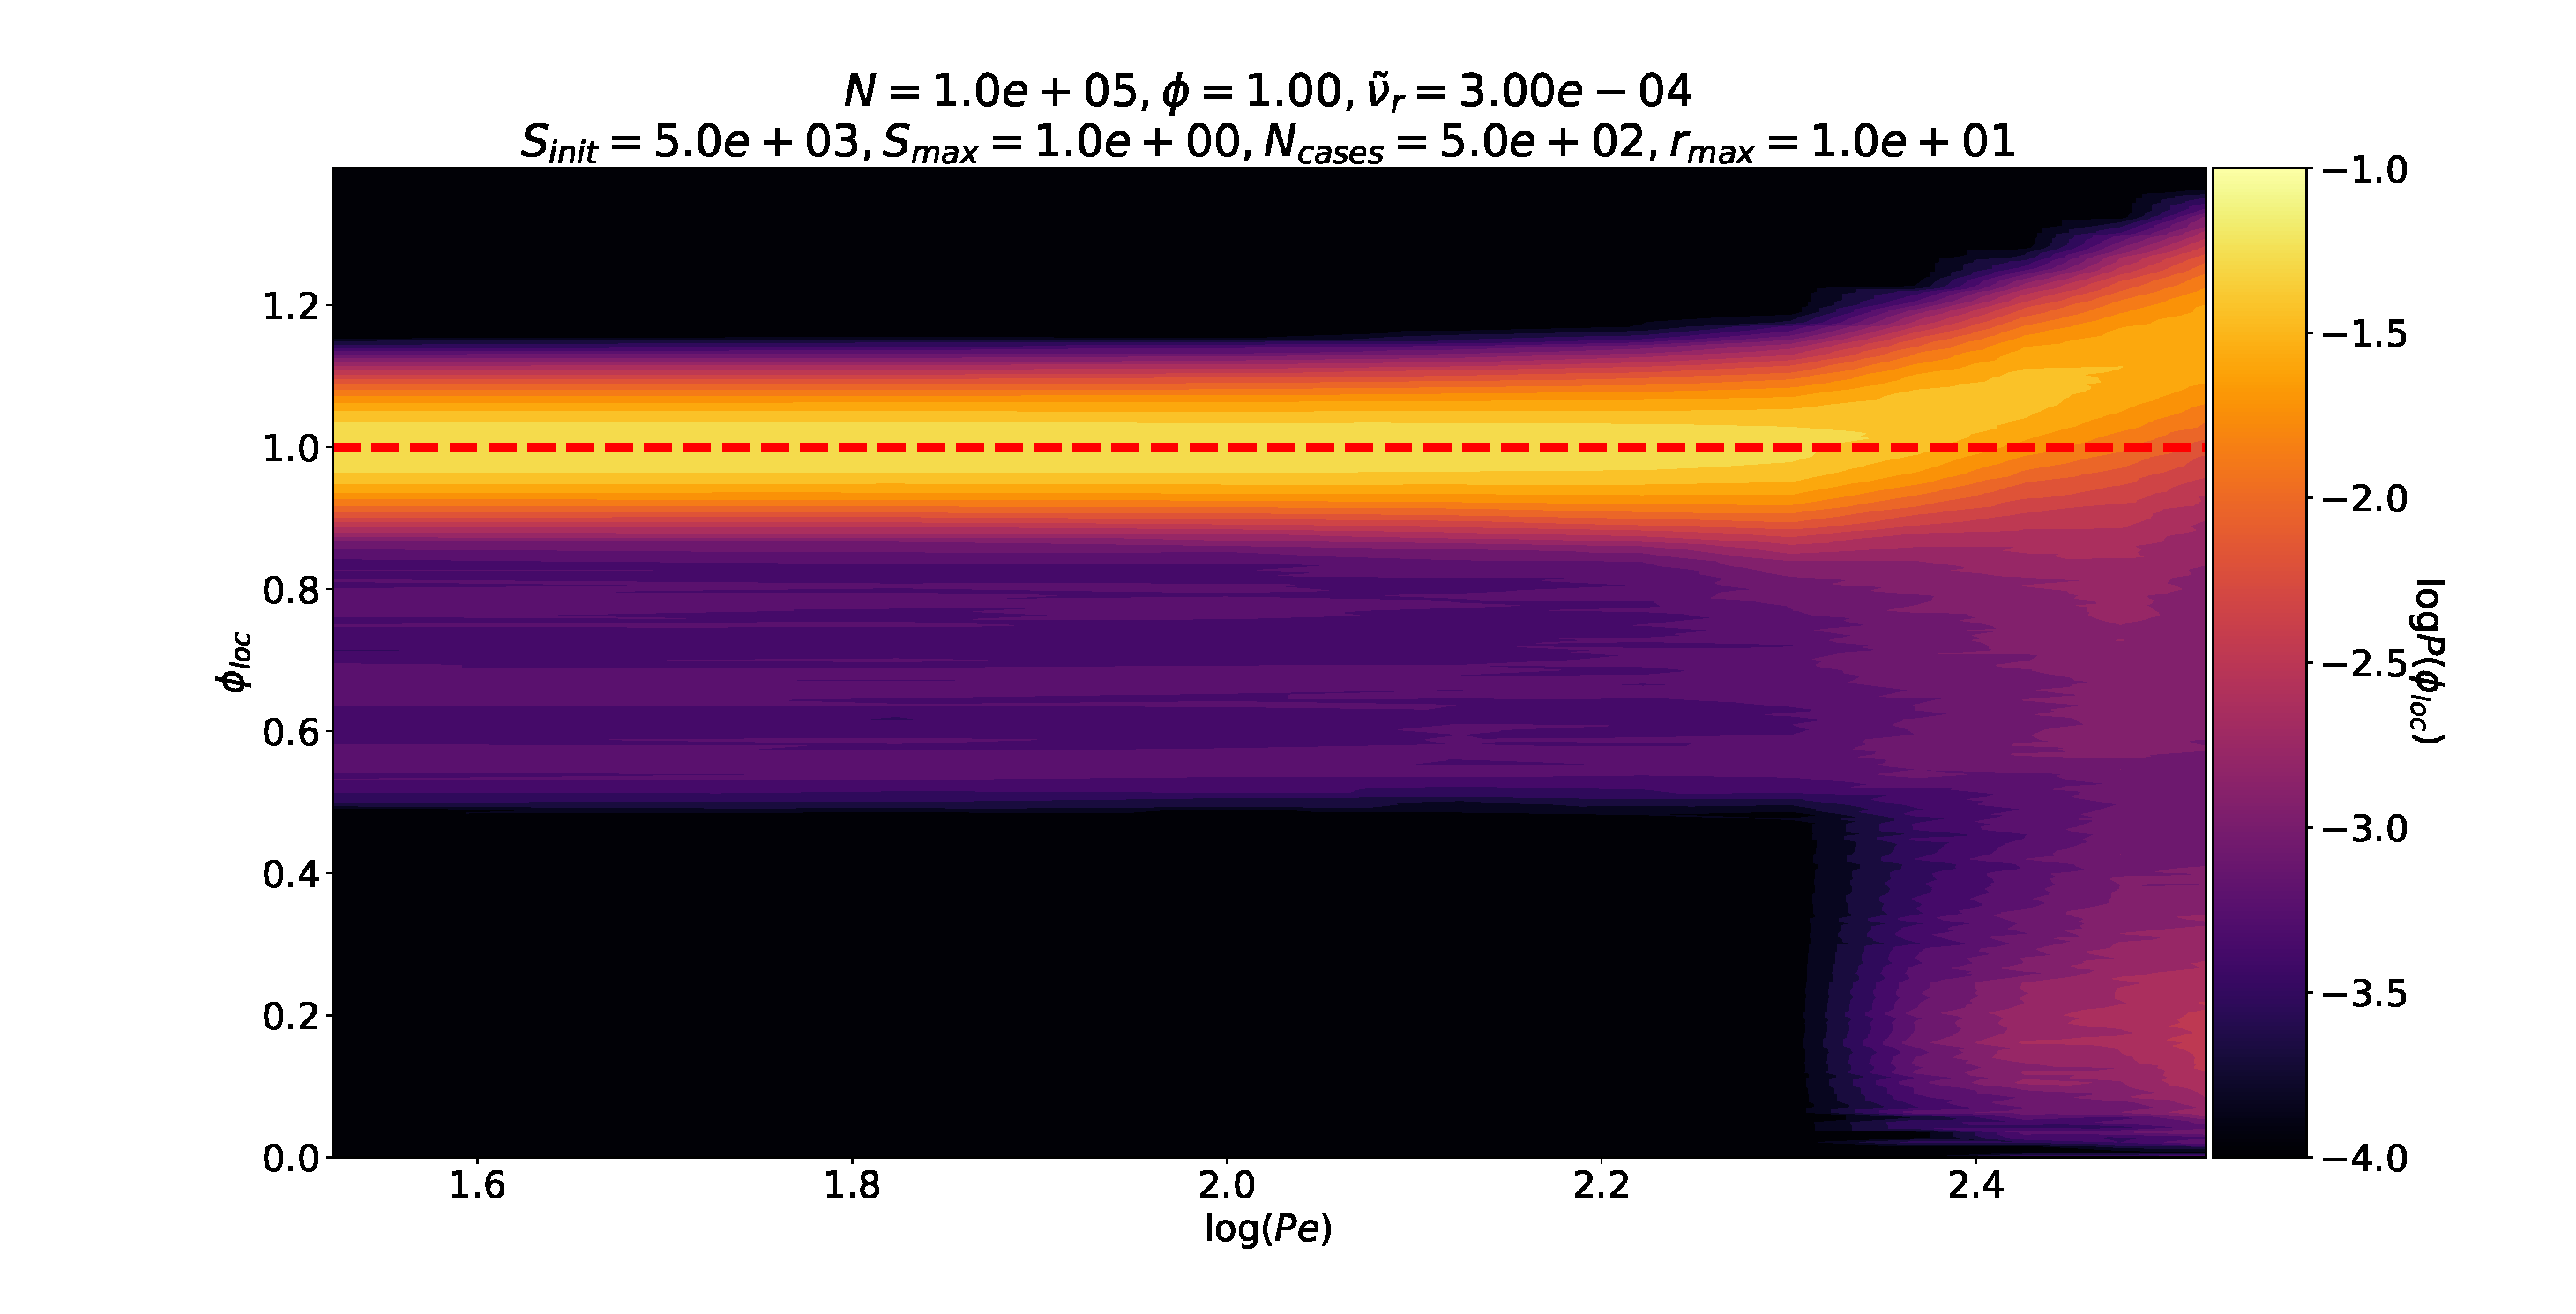
\includegraphics[width=0.9\linewidth]{Pphiloc_Dl1000_Rh3000_Nq1000_Io5000_Ml1000_Cn5000.eps}
  \caption{Histogram of local density $\phi_{loc}$ with varying self-propulsion velocity $\tilde{v}$, at packing fraction $\phi=1.00$ and rotation diffusion constant $\tilde{\nu}_r = 3\cdot10^{-4}$.}
\end{figure}

\end{frame}

\subsection{Displacement correlations and cooperativities}

\begin{frame}{Displacement map at low activity}

\vspace{-0.25cm}
\insertmovie{0.7}{u_Dk8000_Vj1000_Rj1000_Nq1000_Io5000_Tm1000_Bn1000_Pl1000_Mm5000}{Displacement maps at low activity ($\tilde{\nu}_r = 1\cdot10^{-2}$) with $\Delta t = \tau_r$. $\vec{u}(t, t+\Delta t) \equiv$ particle displacement between times $t$ and $t+\Delta t$.}

\end{frame}

\begin{frame}{Displacement map at high activity}

\vspace{-0.25cm}
\insertmovie{0.7}{u_Dk8000_Vj1000_Rg2000_Nq1000_Io5000_Tm5000_Bn1000_Pl5000_Mm5000}{Displacement maps at high activity ($\tilde{\nu}_r = 2\cdot10^{-5}$) with $\Delta t = \tau_r$. $\vec{u}(t, t+\Delta t) \equiv$ particle displacement between times $t$ and $t+\Delta t$.}

\end{frame}

\begin{frame}{Displacement correlation}

$\vec{u}(\vec{r}, t, t + \Delta t) \equiv$ displacement of particle at position $\vec{r}$ between times $t$ and $t + \Delta t$

\begin{align*}
C_{uu}(\Delta \vec{r}, \Delta t) &= \left<\vec{u}(\vec{r}+\Delta\vec{r}, t, t + \Delta t)\cdot\vec{u}(\vec{r}, t, t + \Delta t)\right>_{\vec{r}, t}
\end{align*}

\only<2>{
\begin{align*}
C_{uu}(\Delta \vec{r}, \Delta t) \xrightarrow[\text{isotropy}]{} C_{uu}(\Delta r, \Delta t)
\end{align*}
}

\end{frame}

\begin{frame}{Displacement cooperativity}

\blfootnote{\fullcite{wysocki2014cooperative}}
\blfootnote{\fullcite{doliwa2000cooperativity}}

\begin{align*}
\chi(\Delta t) = \frac{1}{L^2} \int  dr~ 2\pi r~ C_{uu}(r, \Delta t)
\end{align*}
with $L$ the characteristic length of the system.\\

\begin{definition}
$\chi \equiv$ average proportion of particles acting as coherently moving neighbours $\rightarrow$ measure of dynamic heterogeneity.
\end{definition}

\end{frame}

\begin{frame}{Displacement cooperativity with varying $\tilde{\nu}_r$}

\begin{figure}[h!]
  \centering
  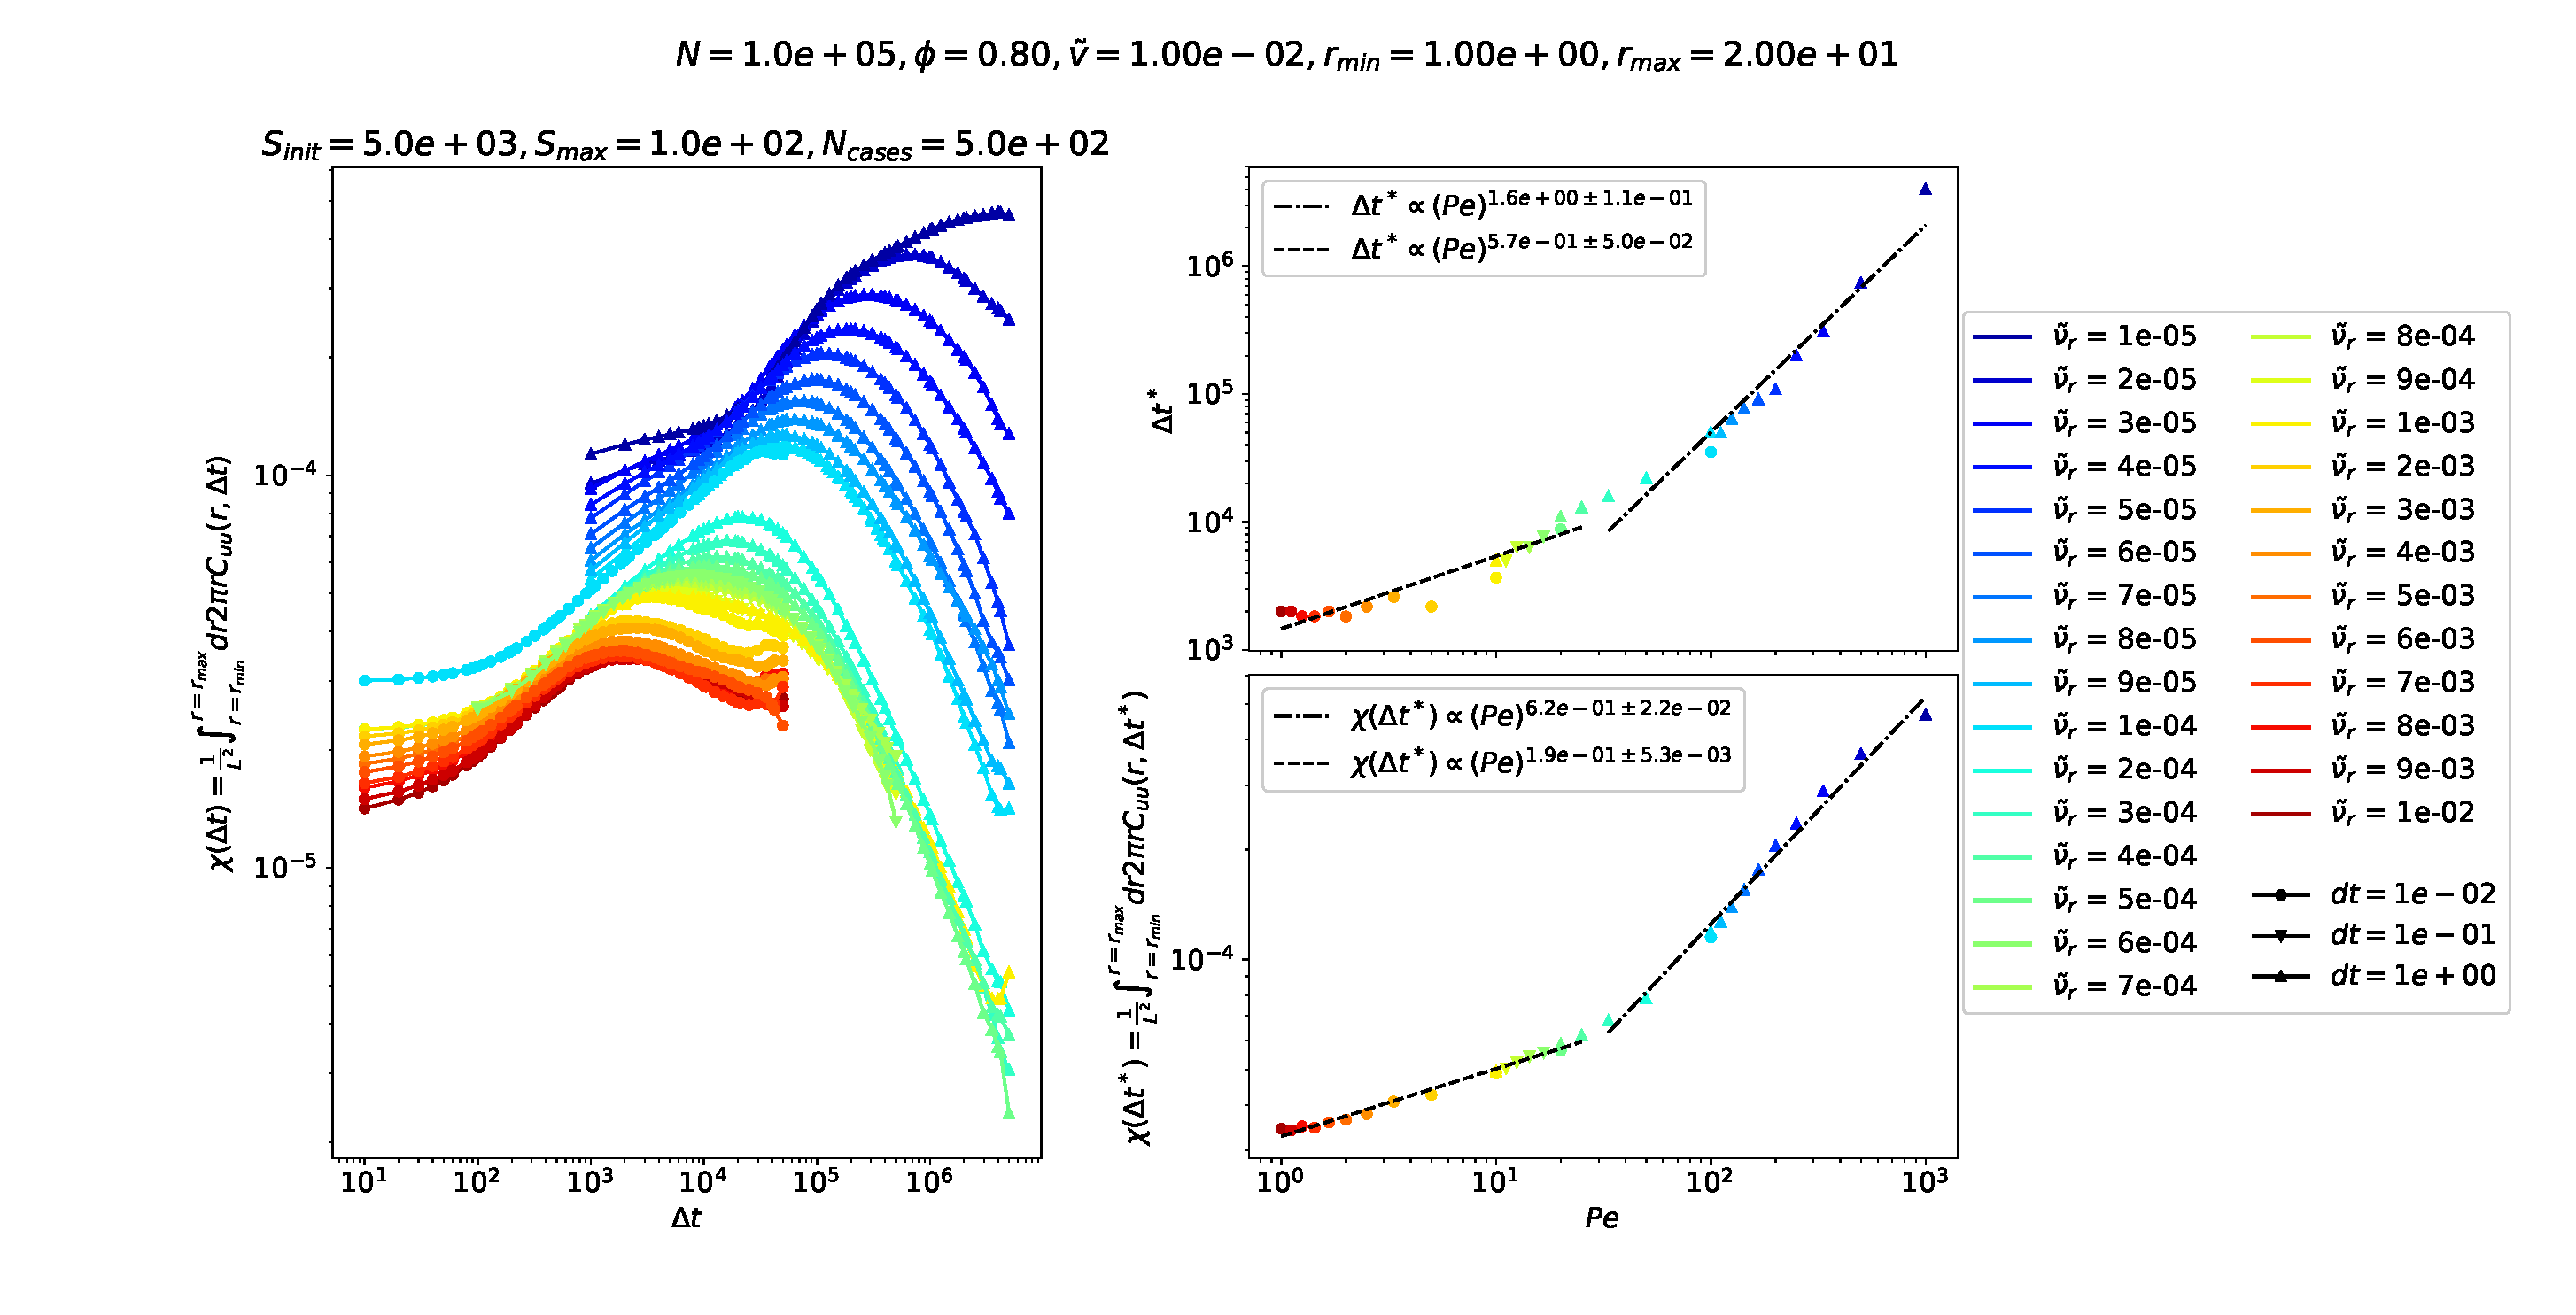
\includegraphics[width=0.9\linewidth]{intCuu_dt_Dk8000_Vj1000_Nq1000_Io5000_Mn1000_Cn5000_RMINl1000_RMAXm2000.eps}
  \vspace{-0.3cm}
  \caption{Comparison of displacement cooperativities $\chi(\Delta t)$, times of maximum cooperativity $\Delta t^*$ and maximum cooperativities $\chi(\Delta t^*)$, at packing fraction $\phi=0.80$ and self-propulsion velocity $\tilde{v}=1\cdot10^{-2}$.}
\end{figure}

\vspace{-0.5cm}
\begin{itemize}
  \item[$\rightarrow$] Clear change of $\Delta t^*(\text{Pe})$ and $\chi(\Delta t^*, \text{Pe})$ slopes at MIPS.
  \item[$\rightarrow$] $(\tau_r \nearrow~ \Leftrightarrow \text{Pe} \nearrow) \Rightarrow \Delta t^* \nearrow,~ \chi(\Delta t^*)\nearrow$
\end{itemize}

\end{frame}

\subsection{Shear strain correlations}

\begin{frame}{Linearised shear strain}

$\vec{u}(\vec{r}, t, t + \Delta t) = \begin{pmatrix} u_x(\vec{r}, t, t + \Delta t) \\ u_y(\vec{r}, t, t + \Delta t) \end{pmatrix} \equiv$ displacement of particle at position $\vec{r}$ between times $t$ and $t + \Delta t$\\

Accumulated shear strain at position $\vec{r}$ between times $t$ and $t  + \Delta t$
\begin{align*}
\varepsilon_{xy}(\vec{r}, t, t + \Delta t) = \frac{1}{2}\left(\frac{\partial}{\partial x}u_y(\vec{r}, t, t + \Delta t) + \frac{\partial}{\partial y}u_x(\vec{r}, t, t + \Delta t)\right)
\end{align*}

\end{frame}

\begin{frame}{Projection of shear strain correlation}

\blfootnote{\fullcite{illing2016strain}}

\begin{align*}
C_{\varepsilon_{xy}\varepsilon_{xy}}(\Delta \vec{r}, \Delta t) &= \left<\varepsilon_{xy}(\vec{r}+\Delta\vec{r}, t, t + \Delta t)\varepsilon_{xy}(\vec{r}, t, t + \Delta t)\right>_{\vec{r}, t}
\end{align*}

\only<2->{
\begin{align*}
C_4^4(\Delta r, \Delta t) &= \frac{1}{\pi} \int_0^{2\pi} d\theta~ \cos(4\theta)~ C_{\varepsilon_{xy}\varepsilon_{xy}}(\Delta\vec{r}\equiv(\Delta r, \theta), \Delta t)
\only<3>{
\\
&\propto \frac{1}{\Delta r^2}\qquad\text{(elastic medium)}
}
\end{align*}
}

\end{frame}

\begin{frame}{Shear strain map at high activity (real space method)}

\vspace{-0.2cm}
\begin{figure}[h!]
  \centering
  \includegraphics[width=0.85\linewidth]{Cssb_Dk8000_Vj1000_Rg2000_Nq1000_Io5000_Tl1000_Ml1000_Cn5000_RCUTl2000_SIGMl2000.eps}
  \vspace{-0.6cm}
  \caption{Shear strain map $\varepsilon_{xy}(\vec{r}, t, t + \Delta t)$ and corresponding shear strain correlations $C_{\varepsilon_{xy}\varepsilon_{xy}}(\Delta\vec{r}, \Delta t)$, at packing fraction $\phi=0.80$, self-propulsion velocity $\tilde{v}=1\cdot10^{-2}$ and rotation diffusion constant $\tilde{\nu}_r=2\cdot10^{-5}$.}
\end{figure}

\vspace{-0.5cm}
\begin{itemize}
  \item[$\rightarrow$] Highest strain values at phase interface.
  \item[$\rightarrow$] Quadropular symmetry of shear strain correlations.
\end{itemize}

\end{frame}

\begin{frame}{Collective mean square displacements}

\blfootnote{\fullcite{illing2016strain}}
\blfootnote{\fullcite{leonforte2005continuum}}

\vspace{-1cm}

\begin{align*}
\vec{u}(\vec{r}, t, t + \Delta t) \xrightarrow[\text{Fourier transform}]{} \tilde{\vec{u}}(\vec{k}, t, t + \Delta t)
\end{align*}

\only<2->{
\begin{align*}
C^{\perp}(\vec{k}, \Delta t) &= \left<||\tilde{\vec{u}}_{\perp}(\vec{k}, t, t  +\Delta t) ||^2\right>\\
C^{||}(\vec{k}, \Delta t) &= \left<||\tilde{\vec{u}}_{||}(\vec{k}, t, t  +\Delta t) ||^2\right>
\end{align*}
respectivement the transversal and longitudinal collective mean square displacements (CMSD).
}

\end{frame}

\begin{frame}{CMSD and shear strain correlations}

\blfootnote{\fullcite{illing2016strain}}
\blfootnote{\fullcite{leonforte2005continuum}}

\vspace{-1cm}

\begin{align*}
C_{\varepsilon_{xy}\varepsilon_{xy}}(\Delta \vec{r}, \Delta t) = \mathcal{F}^{-1}\Big\{&-\frac{k_x^2k_y^2}{k^2}\left(C^{\perp}(\vec{k}, \Delta t) - C^{||}(\vec{k}, \Delta t)\right)\\
&+ \frac{k^2}{4}C^{\perp}(\vec{k}, \Delta t)\Big\}(\Delta \vec{r})
\end{align*}

\only<2->{
\begin{align*}
&\subalign{&C^{||}(\vec{k}, \Delta t) = 0 \\ &C^{\perp}(\vec{k}, \Delta t) \propto k^{-2}} \qquad \text{(incompressible glass)}
\end{align*}
}

\end{frame}

\begin{frame}{CMSD at high activity}

\vspace{-0.2cm}
\begin{figure}[h!]
  \centering
  \includegraphics[width=0.8\linewidth]{Cttb_Dk8000_Vj1000_Rg2000_Nq1000_Io5000_Tl1000_Mn1000_Cn5000_Bn3000_XN1500_Yn1500.eps}
  \vspace{-0.8cm}
  \caption{Transversal and longitudinal CMSD, $C^{\perp}(k, \Delta t) \equiv \left<||\tilde{\vec{u}}_{\perp}(\vec{k}, t, t  +\Delta t) ||^2\right>$ and $C^{||}(k, \Delta t) \equiv \left<||\tilde{\vec{u}}_{||}(\vec{k}, t, t  +\Delta t) ||^2\right>$, at packing fraction $\phi=0.80$, self-propulsion velocity $\tilde{v}=1\cdot10^{-2}$ and rotation diffusion constant $\tilde{\nu}_r=2\cdot10^{-5}$.}
\end{figure}

\vspace{-0.5cm}
\begin{itemize}
  \item[$\rightarrow$] $C^{||}(k, \Delta t) \neq 0$.
  \item[$\rightarrow$] $C^{\perp}(k, \Delta t), C^{||}(k, \Delta t) \propto k^{-2}$ for $\sim$ a decade.
\end{itemize}

\end{frame}

\begin{frame}{Projected strain correlations from CMSD at high activity}

\vspace{-0.2cm}
\begin{figure}[h!]
  \centering
  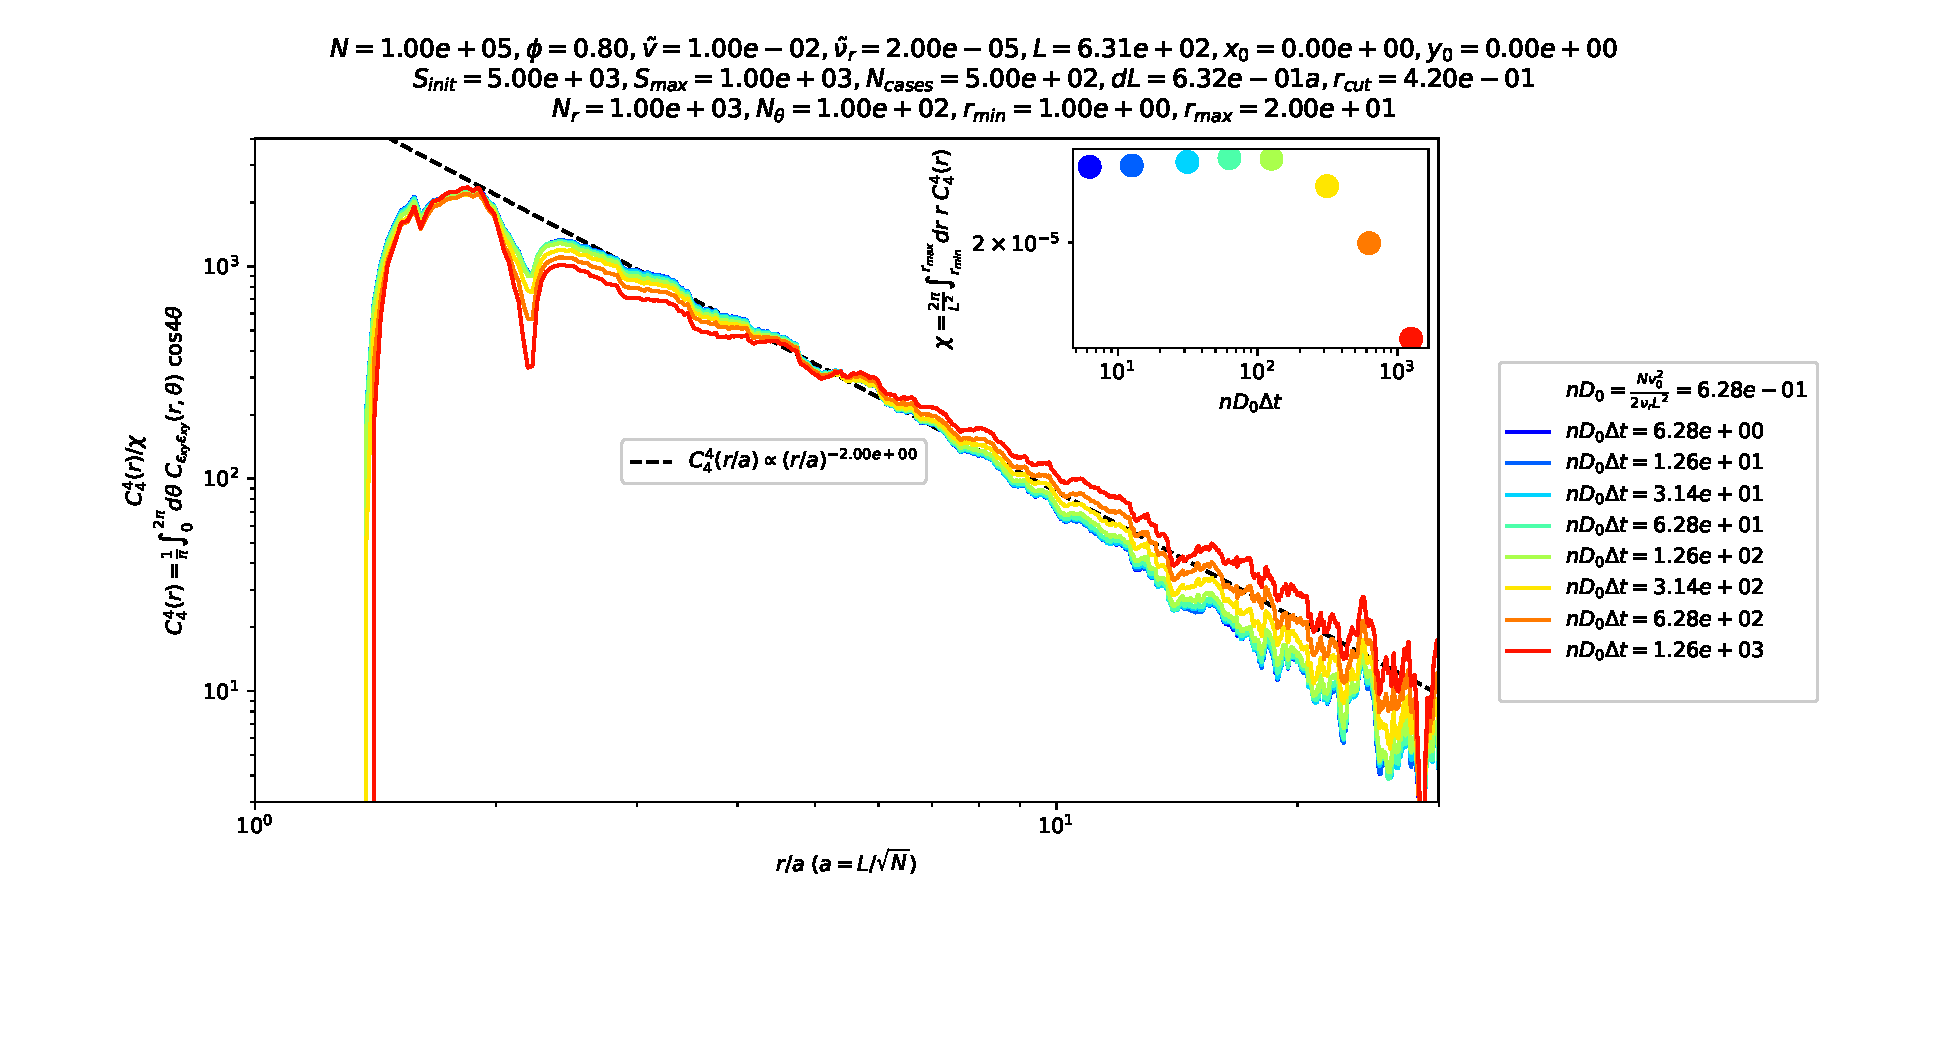
\includegraphics[width=\linewidth]{figures/figs/c44_chi_cmsd_comparison_Dk8000_Vj1000_Rg2000_Nq1000_Ll3000_RCUTk4200_interpolated_loglog.eps}
  \vspace{-1.3cm}
  \caption{Shear strain correlations $C_4^4(\Delta r, \Delta t)$ rescaled by its susceptibility, at packing fraction $\phi=0.80$, self-propulsion velocity $\tilde{v}=1\cdot10^{-2}$ and rotation diffusion constant $\tilde{\nu}_r=2\cdot10^{-5}$.}
\end{figure}

\vspace{-0.8cm}
\begin{itemize}
  \item[$\rightarrow$] Algebraic decay over two decades of lag times.
\end{itemize}

\end{frame}

\begin{frame}{CMSD at low activity}

\vspace{-0.2cm}
\begin{figure}[h!]
  \centering
  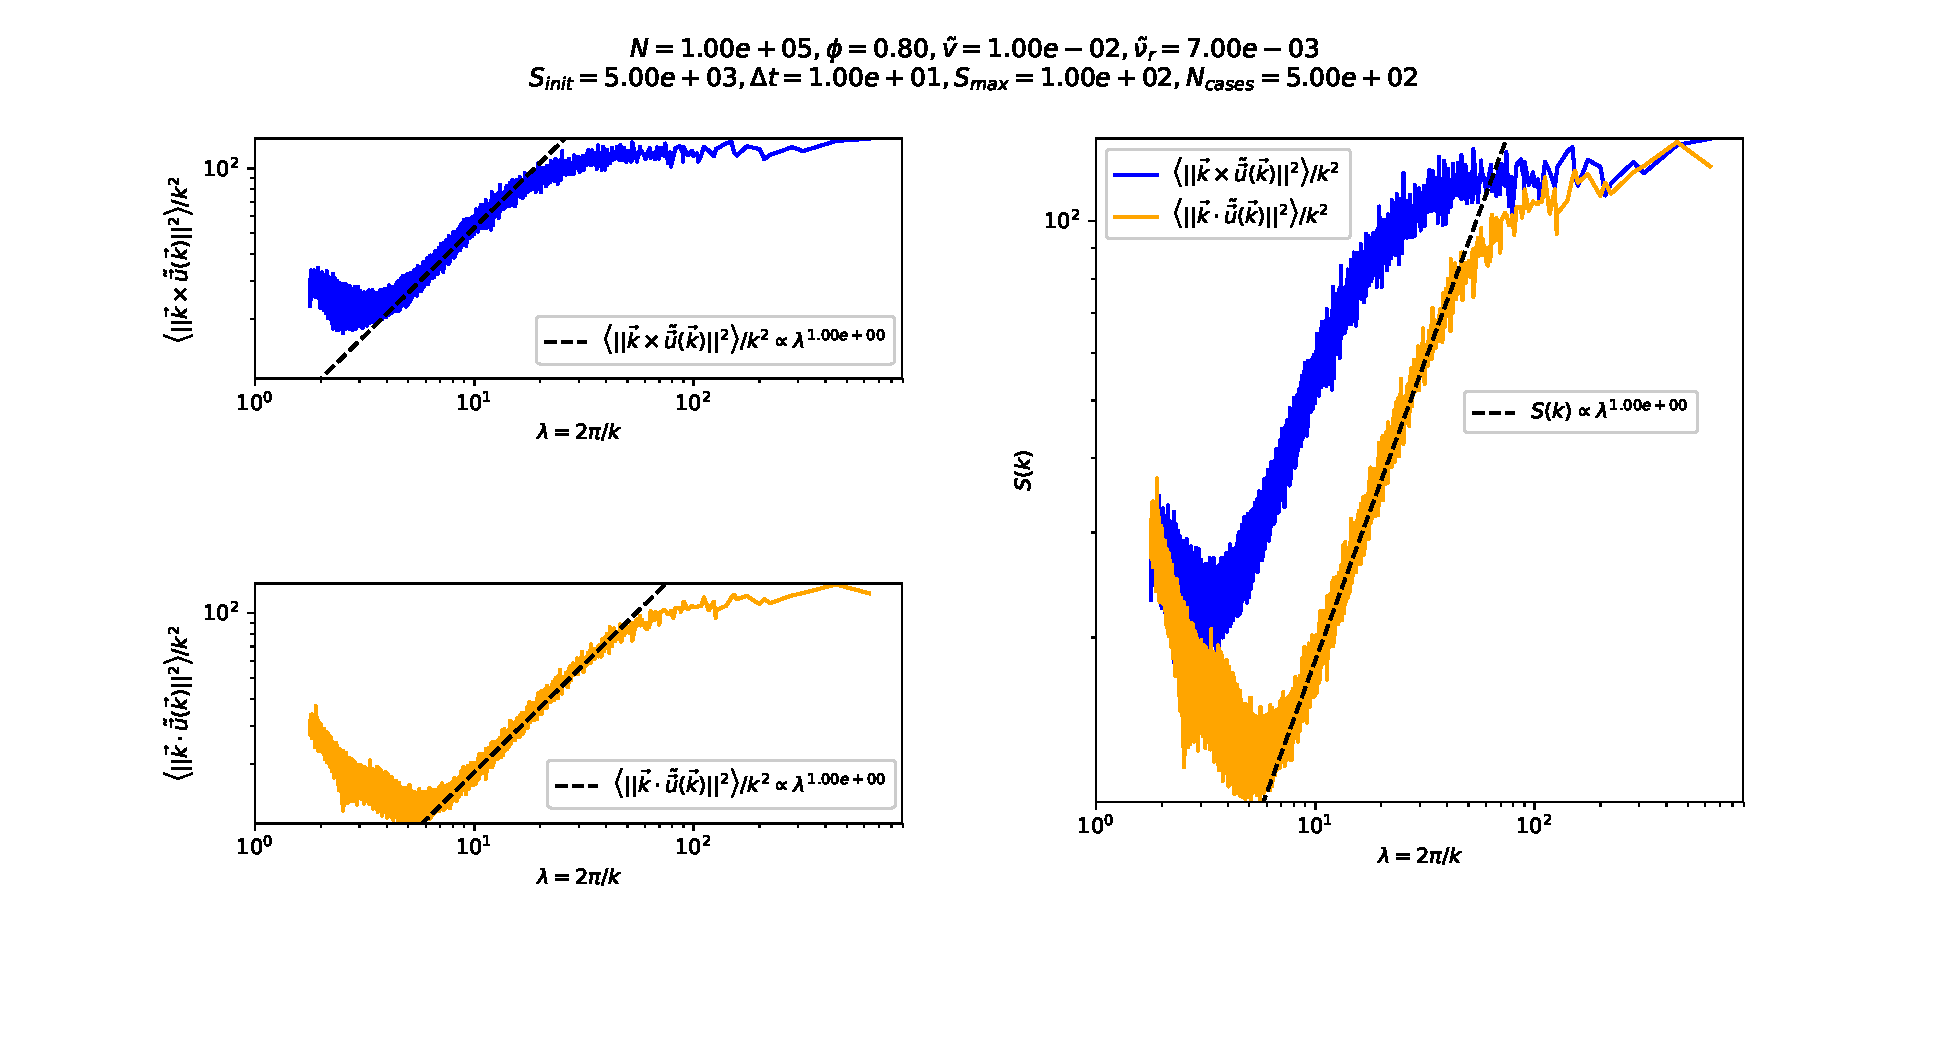
\includegraphics[width=0.85\linewidth]{Cttb_Dk8000_Vj1000_Ri7000_Nq1000_Io5000_Tl1000_Mn1000_Cn5000.eps}
  \vspace{-0.8cm}
  \caption{Transversal and longitudinal CMSD, $C^{\perp}(k, \Delta t) \equiv \left<||\tilde{\vec{u}}_{\perp}(\vec{k}, t, t  +\Delta t) ||^2\right>$ and $C^{||}(\vec{k}, \Delta t) \equiv \left<||\tilde{\vec{u}}_{||}(\vec{k}, t, t + \Delta t) ||^2\right>$, at packing fraction $\phi=0.80$, self-propulsion velocity $\tilde{v}=1\cdot10^{-2}$ and rotation diffusion constant $\tilde{\nu}_r=7\cdot10^{-3}$.}
\end{figure}

\vspace{-0.5cm}
\begin{itemize}
  \item[$\rightarrow$] $C^{\perp}(\vec{k}, \Delta t), C^{||}(k, \Delta t) \propto k^{-1}$ for $\sim$ a decade.
\end{itemize}

\end{frame}

\begin{frame}{Projected strain correlations from CMSD at low activity}

\begin{figure}[h!]
  \centering
  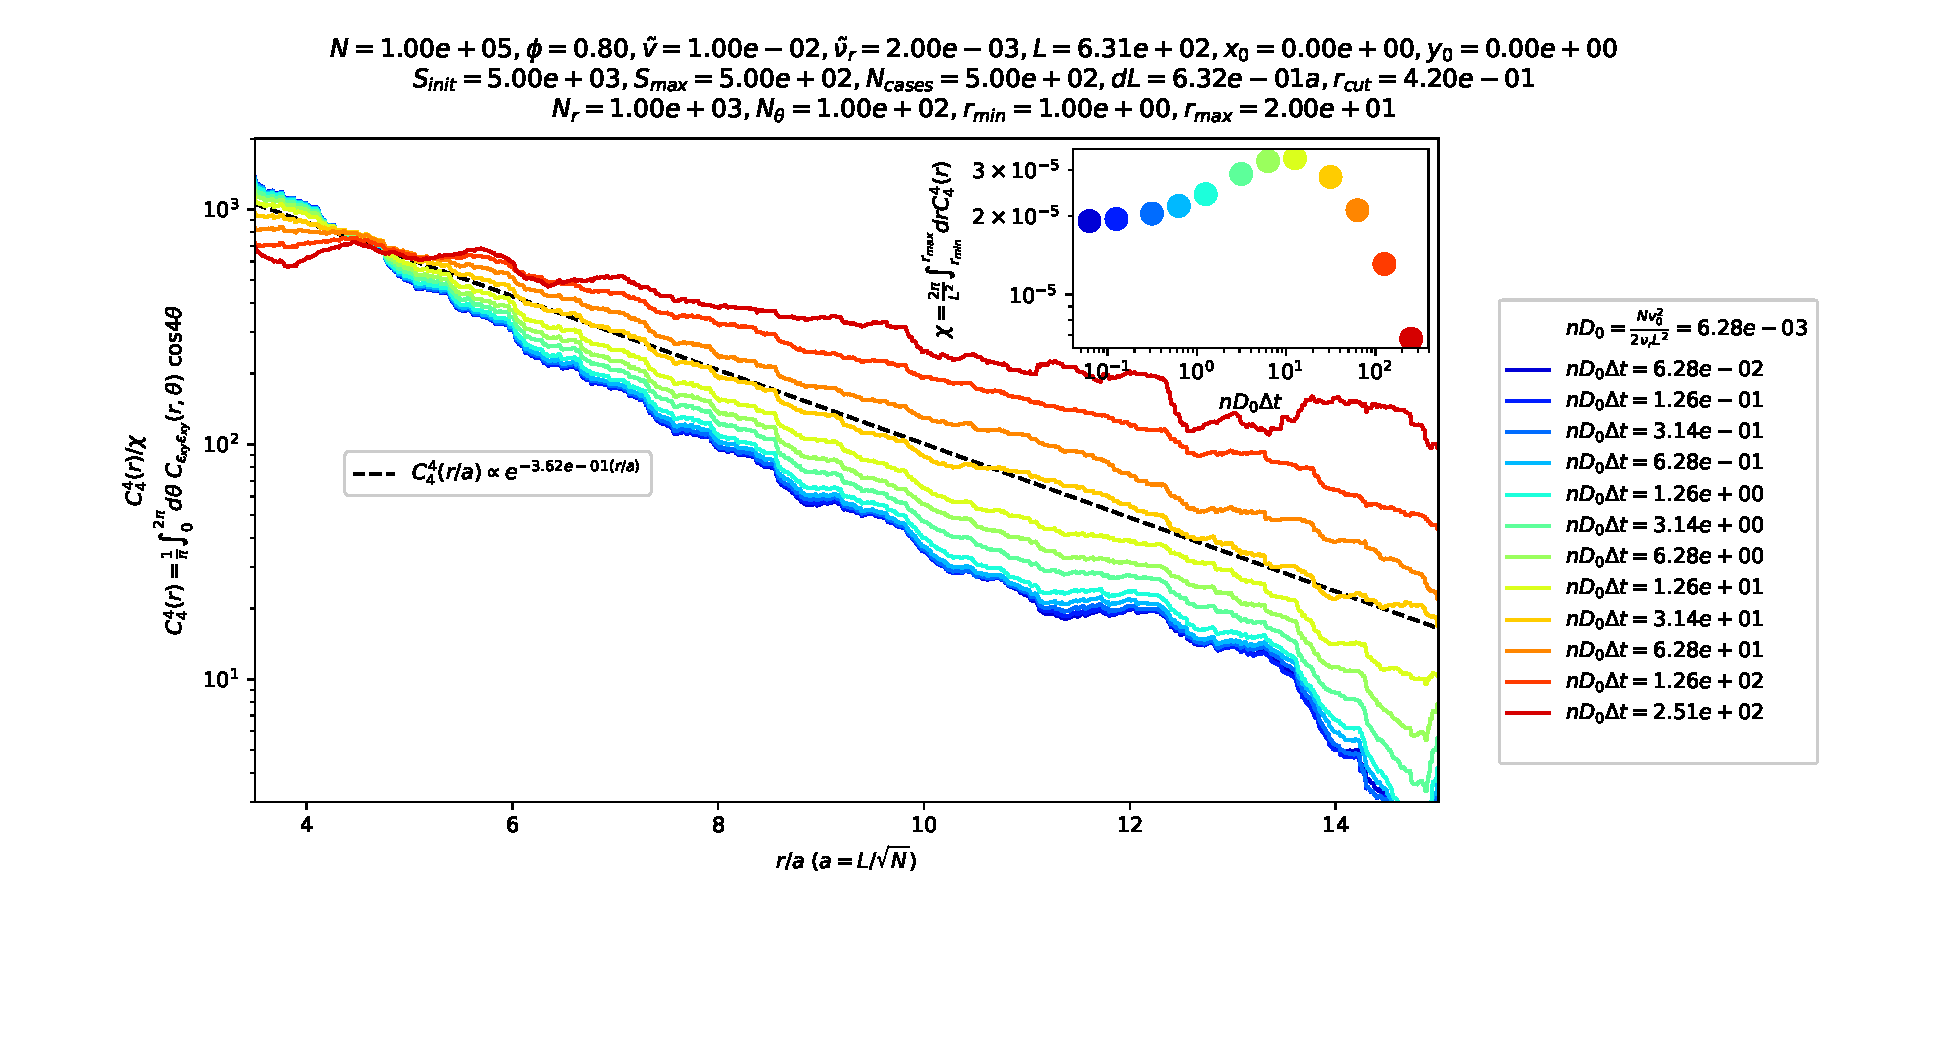
\includegraphics[width=0.95\linewidth]{figures/figs/c44_chi_cmsd_comparison_Dk8000_Vj1000_Ri2000_Nq1000_Ll0000_Mo1000_RCUTk4200_interpolated_linlog.eps}
  \vspace{-1.1cm}
  \caption{Shear strain correlations $C_4^4(\Delta r, \Delta t)$ rescaled by its susceptibility, at packing fraction $\phi=0.80$, self-propulsion velocity $\tilde{v}=1\cdot10^{-2}$ and rotation diffusion constant $\tilde{\nu}_r=2\cdot10^{-3}$.}
\end{figure}

\vspace{-0.8cm}
\begin{itemize}
  \item[$\rightarrow$] Exponential decay at all lag times.
  \item[$\rightarrow$] Exponential decay length scale around $2a$ and increasing function of lag time.
\end{itemize}

\end{frame}

\section{Conclusion}

\begin{frame}{Conclusion}

\begin{itemize}
\item Active matter system displaying motility-induced phase separation.
\only<2->{
\item At fixed self-propulsion velocity, this transition is accompanied by increased cooperativity $\Rightarrow$ increased dynamic heterogeneity.
}
\only<3->{
\item Shear strain correlations show algebraic decay for phase-separated systems and exponential decay for homogenous fluid systems.
}
\end{itemize}

\end{frame}

\begin{frame}{Outlook}

\begin{itemize}
\item Explore other paths through phase space to understand variations of cooperativities.
\only<2>{
\item Characterise the transition from exponential to algebraic decay in shear strain correlations.
}
\end{itemize}

\end{frame}

\end{document}
